\makeatletter\let\ifGm@compatii\relax\makeatother
\documentclass[red]{beamer}

%\usepackage{beamerthemesplit}
\usepackage{listings}
\usepackage{comment}
\usepackage{url}
\usepackage{bm}
\usepackage{todonotes}
\usepackage{tikz}
\usetikzlibrary{arrows.meta}
\usetikzlibrary{shapes.symbols}

\usepackage{hyperref} % has to be last
\hypersetup{
    colorlinks=true,
    linkcolor=blue,
    filecolor=magenta,      
    urlcolor=cyan,
    pdfpagemode=FullScreen,
    }

\tikzset{
    saiarrow/.style={{-Latex}, thick}
}

\newcommand{\isred}[1]{{\color{red} {\bf #1}}} 
\newcommand{\isblue}[1]{{\color{blue}{\bf #1}}} 
\newcommand{\isgreen}[1]{{\color{green} {#1}}} 
\newcommand{\isdarkgreen}[1]{{\color{darkgreen} {#1}}} 
\newcommand{\isorange}[1]{{\color{orange} {#1}}} 

\begin{document}


\setbeamercolor{alerted_text}{fg=cyan}
\xdefinecolor{purplish}{cmyk}{0.75,0.75, 0, 0}
\xdefinecolor{purple}{cmyk}{0.75,0.75, 0, 0}
\colorlet{newred}{red!60!black}

\title{Session 1: Introduction to Protocol Security}
\author{Slides prepared by UMBC Protocol Analysis Lab}
\date{Last edited \today}
\maketitle

\begin{frame}\frametitle{What is the goal of this course}
\pause
To teach students how to verify cryptographic network protocols.

\pause
To introduce students to the UMBC Protocol Analysis Lab (PAL).

\pause
To teach students how to use the Cryptographic Protocol Shapes analyzer (CPSA).

\pause
To teach students adversarial thinking.

\end{frame}


\begin{frame}\frametitle{Meet your instructors}
\vspace{1em}
\begin{columns}
\pause
    \column{0.3\textwidth}
    \vspace{-2em}
    \begin{block}{\small Michael Barthel}
        \small Rising Junior in PAL.
        
        \small Digital provenance \\ and fintech.

        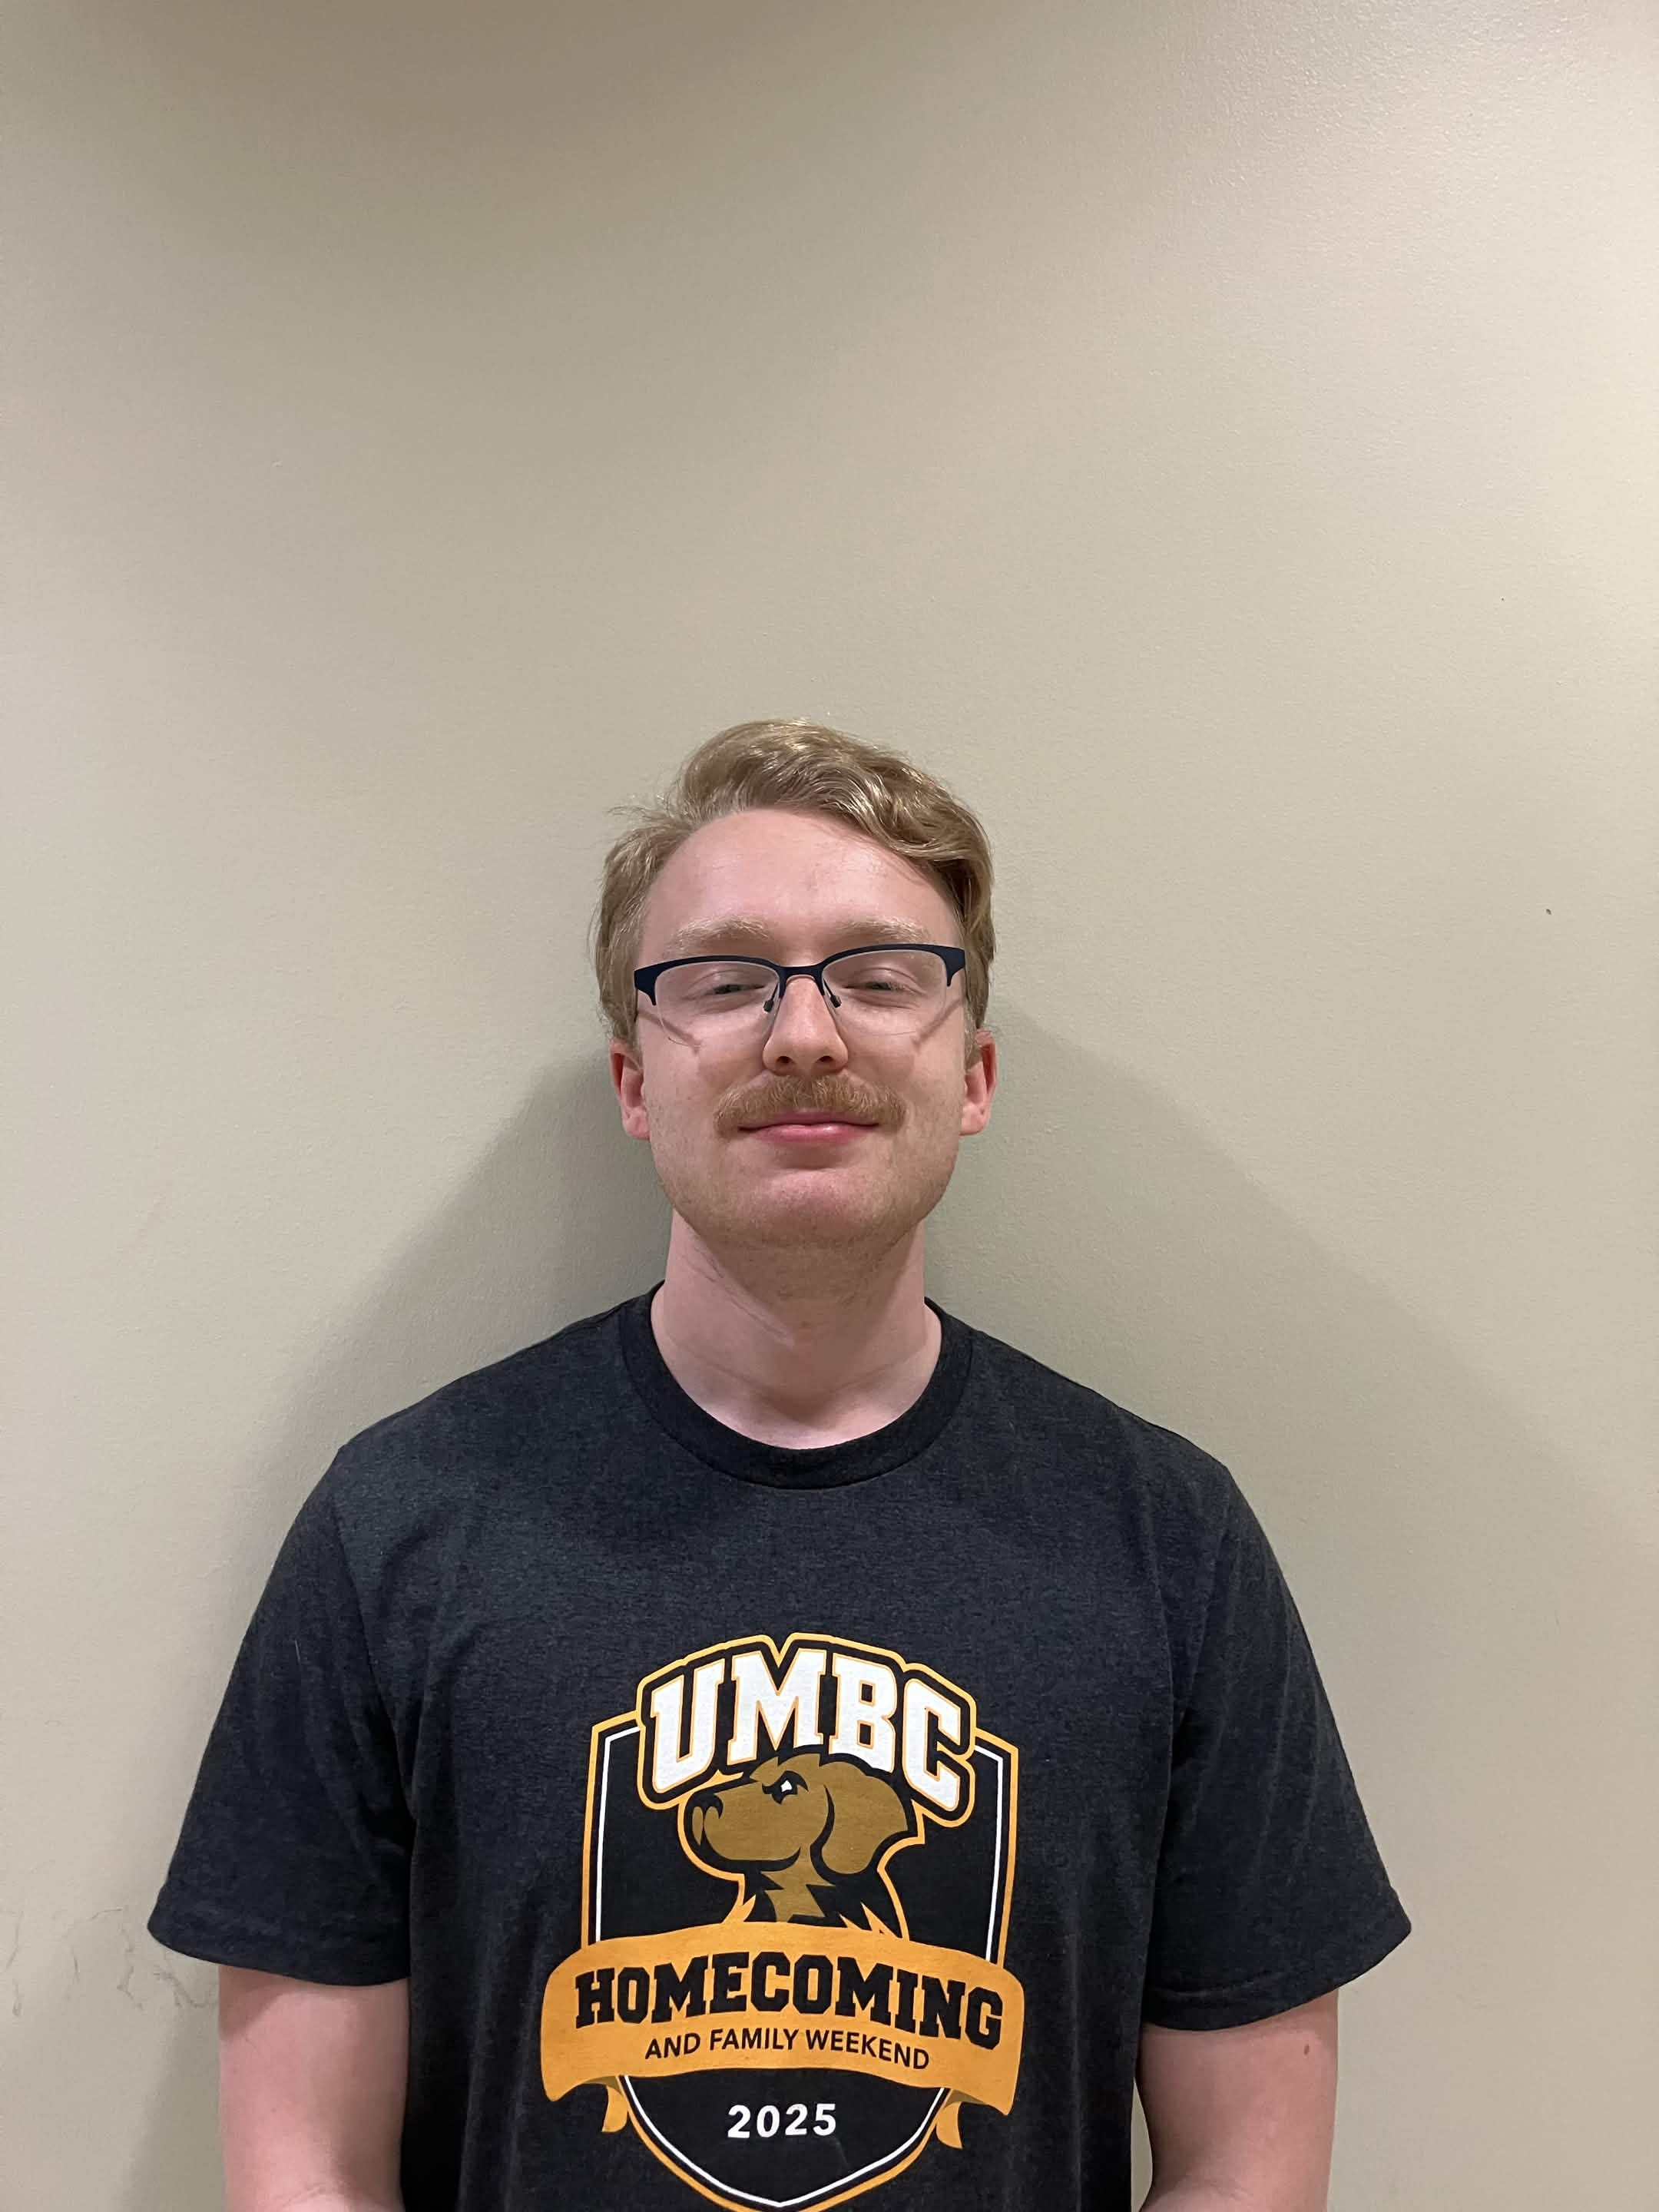
\includegraphics[height=0.28\textheight]{slide-images/michael}
    \end{block}
\pause
    \column{0.3\textwidth}
    \vspace{-2em}
    \begin{block}{\small Sai Matukumalli}
        \small Graduate from PAL.
        \small Mathematical cryptography and complexity.

        \includegraphics[height=0.22\textheight]{slide-images/sai}
    \end{block}
\pause
    \column{0.3\textwidth}
    \vspace{-1.5em}
    \begin{block}{\small Ceridwen Summerlot}
        \small Rising Junior in PAL. \\
        \small Education and website development. \\
        \includegraphics[height=0.25\textheight]{slide-images/ceridwen.jpg}
        \end{block}
\end{columns}

\vspace{0.25cm}

% Second row
\begin{columns}
\pause
    \column{0.3\textwidth}
    \vspace{-1.5em}
    \begin{block}{\small DeMarko Fulcher}
        \small Graduate from PAL.
        
        \small Formal verification.

        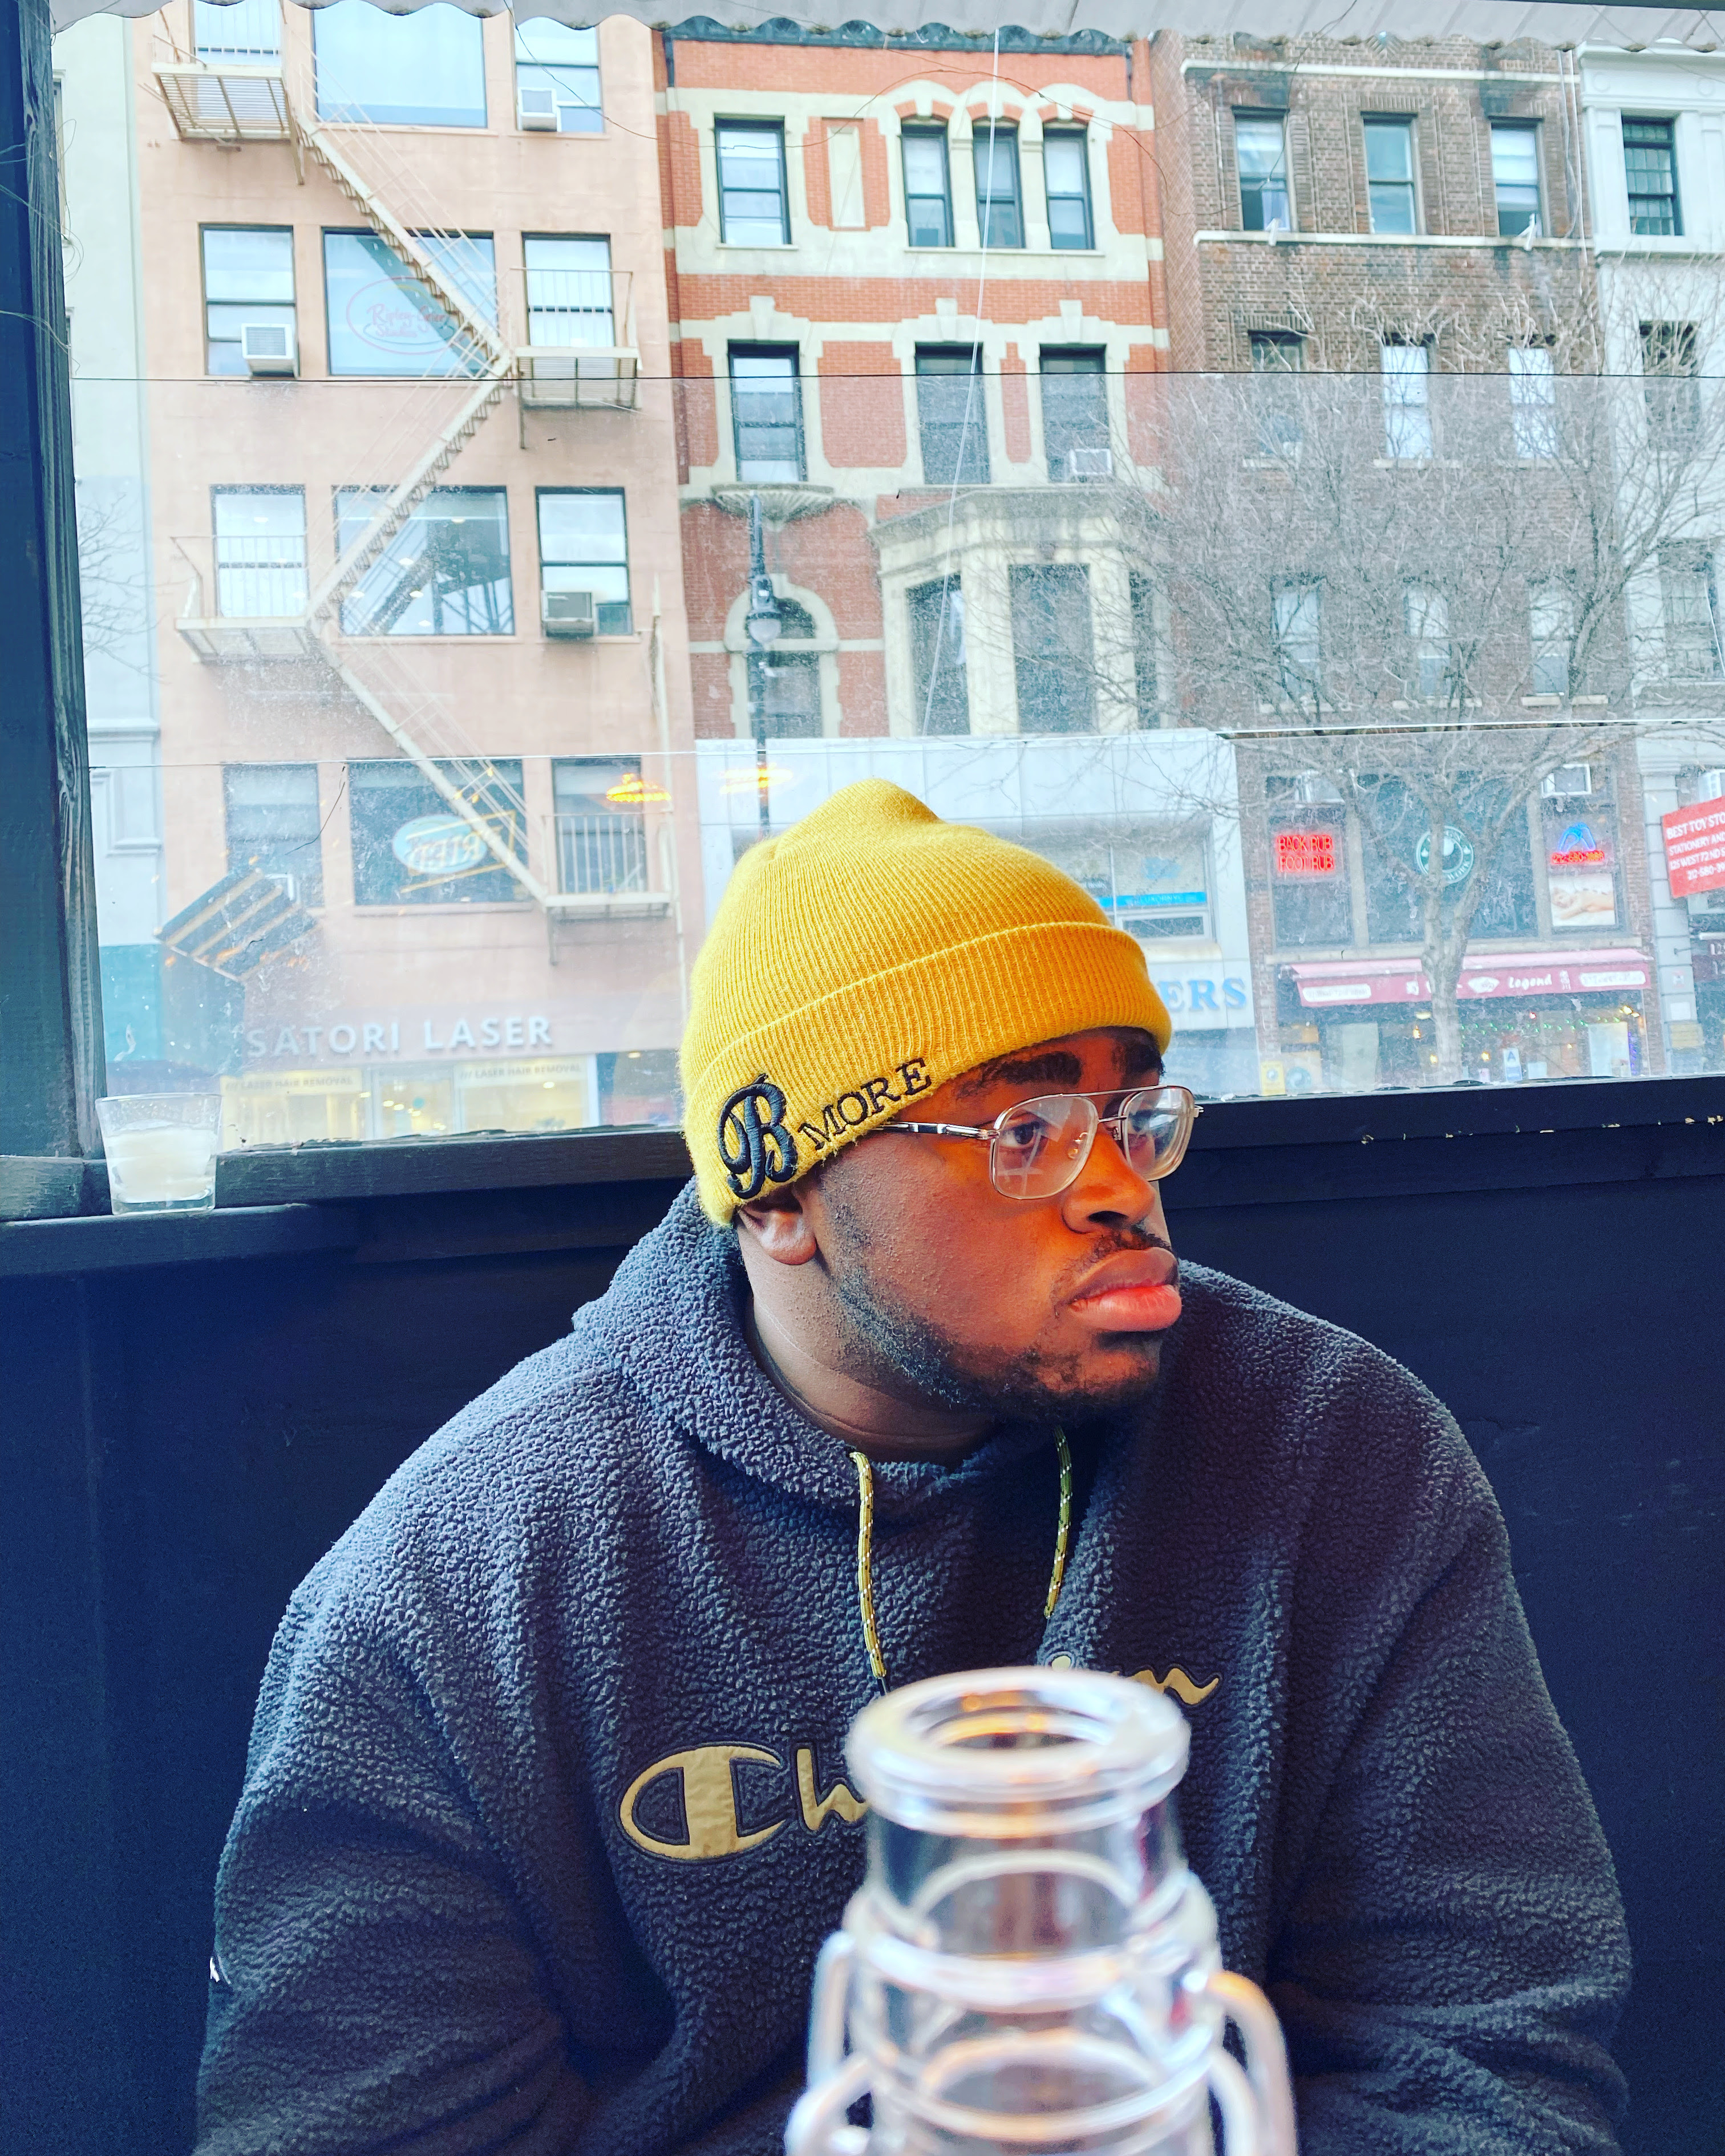
\includegraphics[height=0.25\textheight]{slide-images/demarko}
    \end{block}
\pause
    \column{0.3\textwidth}
    \vspace{-1.5em}
    \begin{block}{\small Jeremy Romano}
        \small Graduate from PAL. \\
        \small Implementation of attacks. \\
        \includegraphics[height=0.25\textheight]{slide-images/jeremy}
        \end{block}
\pause
    \column{0.3\textwidth}
    \vspace{-1.5em}
    \begin{block}{\small Dr.\ Enis Golaszewski}
        \small PI of PAL. \\
        \small Everything everyone else does and more. \\
        \includegraphics[height=0.25\textheight]{slide-images/enis}
        \end{block}
\end{columns}

\end{frame}

\begin{frame}\frametitle{Meet your classmates}
\pause
Introduce yourselves!
\pause
We will start with people in person, and then go online.

\pause
These are your classmates for the entire month, you should try to learn everyone's names.

\pause
There will be a final project that you can work in groups on, so you should try and find some people that you are interested in working with.

\pause

\end{frame}


\title{Introduction to Protocols}
\author{How do Alice and Bob communicate?}
\date{}
\begin{frame}
\maketitle
\end{frame}

\begin{frame}\frametitle{What is a protocol}
\begin{itemize}
\pause
\item Exchange of messages between two or more parties
\pause
\item Follows a set of well-defined instructions
\pause
\item Network communication occurs through protocols
\end{itemize}
\end{frame}


\begin{frame} \frametitle{Where do we encounter protocols?}
\begin{itemize}
\pause
\item Everywhere!
\pause
\item Day-to-day life: Personal, business
\pause
\item Computer networks: HTTP, VoIP, TCP, etc.
\pause
\begin{itemize}
\item These are generally not visible to the user, but are important!
\end{itemize}
\end{itemize}
\end{frame}

\begin{frame}\frametitle{What does a protocol look like?}
\pause
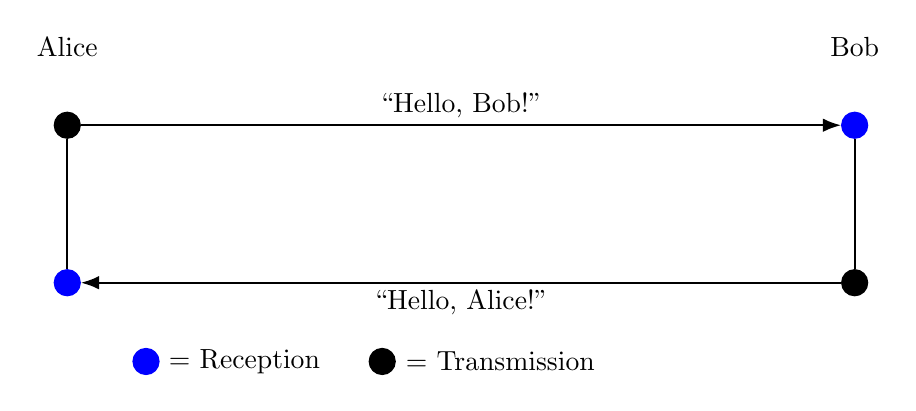
\begin{tikzpicture}
    \node at (0,8) {Alice};
    \node at (10,8) {Bob};
    \node[shape=circle,draw=blue, fill=blue] at (1,4) {};
    \node at (2.25,4) {= Reception};
    \node[shape=circle,draw=black, fill=black] (1) at (4,4) {};
    \node at (5.5,4) {= Transmission};

    \pause
    \node[shape=circle,draw=black, fill=black] (4) at (0,7) {};

    \pause
    \node[shape=circle,draw=blue, fill=blue] (3) at (10,7) {};
    \path [saiarrow](4) edge (3);
    \node at (5,7.25) {``Hello, Bob!''};
    
    \pause
    \node[shape=circle,draw=black, fill=black] (2) at (10,5) {};
    \path [-,thick](3) edge (2);
    
    \pause
    \node[shape=circle,draw=blue, fill=blue] (1) at (0,5) {};
    \path [saiarrow](2) edge (1);
    \node at (5,4.75) {``Hello, Alice!''};
    \path [-,thick](1) edge (4);
    \pause
\end{tikzpicture}
\bigskip
\end{frame}



%%%%%%%%%%%%%%%%%%%%%%%%%%%%%%%%%%%%%%%%%%%%%%%%%%%%%%%%%%%%%%%%%%%%%%%%%%%%%%%%%%%%%%%%%%%%%%%%%%%%%%%

\title{Why cryptographic protocols?}
\author{When do we need to take steps to protect communication between parties?}
\date{}
\begin{frame}
\maketitle
\end{frame}

\begin{frame}\frametitle{What is the problem space?}
\pause
We start with a simple problem.

\pause
\isred{Problem:} Alice and Bob want to set up a meeting without Charlie finding out, how do they do it?

\pause
Can you think of some na\"ive solutions?

\pause
\begin{enumerate}
\item Alice can tell Bob about the meeting in another language, one that Charlie doesn't know?
\pause
\item Alice can hide information about the meeting in random places that Bob knows to check?
\pause
\item Alice and Bob can go somewhere that they're sure that no one is around, and then talk about the meeting?
\pause
\item [] Other ideas?
\end{enumerate}
\end{frame}

\begin{frame}\frametitle{What can we do?}
\pause
How can we turn these na\"ive solutions into concrete concepts.
\pause
Eventually -- turn these ideas into mathematical statements.
\pause
\begin{enumerate}
\item A secret language requires both the sender and receiver to have a ``key'', that lets them understand how words correspond to things.

\pause
\item Hiding information corresponds to presharing information, and using a combination of presharing and given information, Bob can derive information.

\pause
\item Alice and Bob making sure no one is around is like an airgap. Can they really be sure \emph{no one} is listening?

\pause
\end{enumerate}
\end{frame}

%%%%%%%%%%%%%%%%%%%%%%%%%%%%%%%%%%%%%%%%%%%%%%%%%%%%%%%%%%%%%%%%%%%%%%%%%%%%%%%%%%%%%%%%%%%%%%%%


\title{Why is Protocol Security Challenging?}
\author{If we can do all these actions, can't we make our protocol secure?}
\date{}
\begin{frame}
\maketitle
\end{frame}


\begin{frame}\frametitle{Why is Protocol Security Challenging?}
\begin{itemize}
\pause
\item Protocols often have security goals.
\begin{itemize}
\item Confidentiality
\item Integrity
\item Authenticity
\item[]
\item We will talk about these next time
\end{itemize}
\pause
\item There is an adversary.
\end{itemize}

\end{frame}

\begin{frame}\frametitle{The Dolev-Yao Network Intruder}
\begin{itemize}
\item Dolev, D.; Yao, A. C. (1983), \href{http://www.cs.huji.ac.il/~dolev/pubs/dolev-yao-ieee-01056650.pdf}{``On the security of public key protocols''}
\item “The attacker carries the messages.”
\item ASSUMPTION: Adversary cannot break cryptographic functions.
\end{itemize}
\end{frame}

\begin{frame}\frametitle{Is this really what a network looks like?}
\pause
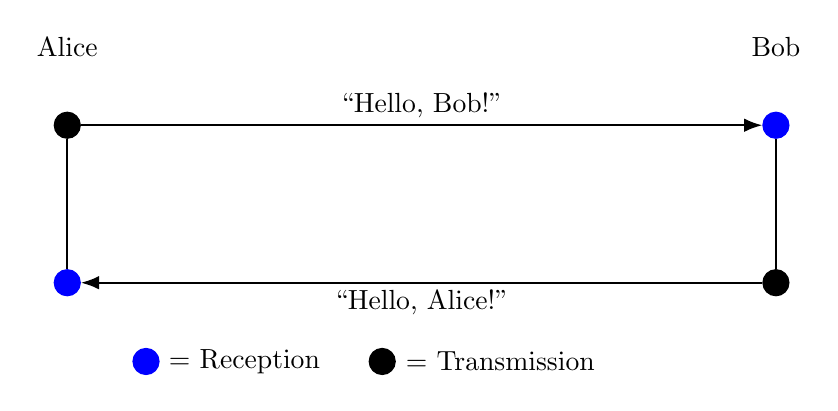
\begin{tikzpicture}
    \node at (0,8) {Alice};
    \node[shape=circle,draw=blue, fill=blue] (1) at (0,5) {};
    \node[shape=circle,draw=black, fill=black] (4) at (0,7) {};
    \node at (4.5,7.25) {``Hello, Bob!''};

    \node at (9,8) {Bob};
    \node[shape=circle,draw=black, fill=black] (2) at (9,5) {};
    \node[shape=circle,draw=blue, fill=blue] (3) at (9,7) {};
    \node at (4.5,4.75) {``Hello, Alice!''};

    \path [saiarrow](2) edge (1);
    \path [-,thick](3) edge (2);
    \path [saiarrow](4) edge (3);
    \path [-,thick](1) edge (4);

    \node[shape=circle,draw=blue, fill=blue] at (1,4) {};
    \node at (2.25,4) {= Reception};
    \node[shape=circle,draw=black, fill=black] (1) at (4,4) {};
    \node at (5.5,4) {= Transmission};
\end{tikzpicture}
\bigskip

\centering
\textbf{Does this really reflect what a network looks like?}
\end{frame}

\begin{frame}\frametitle{An adversarial model of the network}
\pause
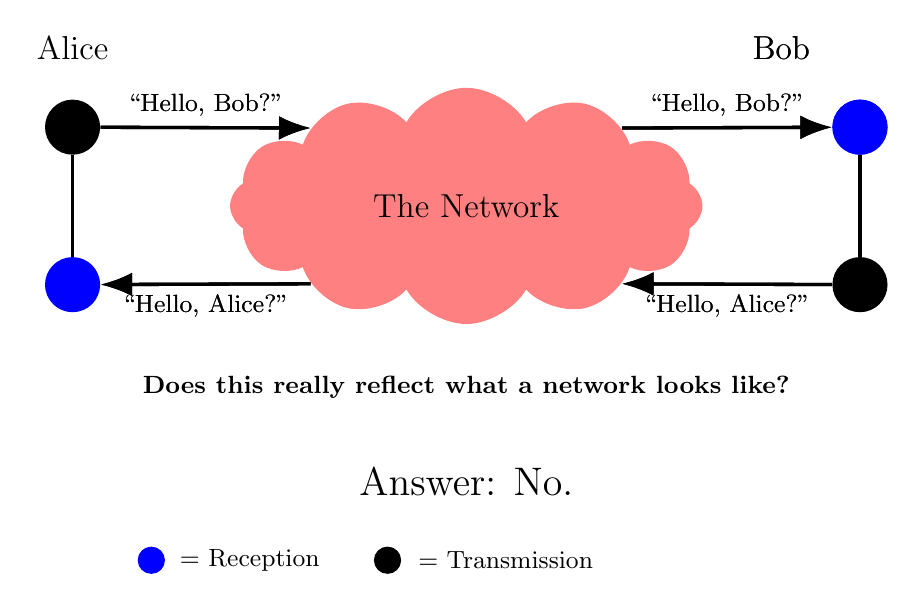
\begin{tikzpicture}[
    node distance=2cm,
    every node/.style={font=\small},
    dot/.style={circle, minimum size=0.7cm, inner sep=0pt},
    arrow/.style={-{Latex[length=4mm]}, very thick}
]

    % Left side (Alice)
    \node at (0,4.5) {\large Alice};
    % Right side (Bob)
    \node at (9,4.5) {\large Bob};
    % Network cloud
    \node[cloud, cloud puffs=12, cloud puff arc=120,
          aspect=2, draw=none, fill=red!50, minimum width=6cm, minimum height=3cm]
          (net) at (5,2.5) {\large The Network};
    
    \pause 
    \node[dot, fill=black] (A1) at (0,3.5) {};
    \node[shape=circle,draw=blue, fill=blue] at (1,-2) {};
    \node at (2.25,-2) {= Reception};
    \node[shape=circle,draw=black, fill=black] (1) at (4,-2) {};
    \node at (5.5,-2) {= Transmission};
    
    \pause
    \draw[arrow] (A1) -- node[above] {``Hello, Bob?''} (net.north west);
    
    \pause 
    \node[dot, fill=blue]  (B1) at (10,3.5) {};
    
    \pause
    \draw[arrow] (net.north east) -- node[above] {``Hello, Bob?''} (B1);
    
    \pause 
    \node[dot, fill=black] (B2) at (10,1.5) {};
    \draw[very thick] (B1) -- (B2);
    
    \pause
    \draw[arrow] (B2) -- node[below] {``Hello, Alice?''} (net.south east);
    
    \pause 
    \node[dot, fill=blue]  (A2) at (0,1.5) {};
    
    \draw[very thick] (A1) -- (A2);
    
    \pause
    \draw[arrow] (net.south west) -- node[below] {``Hello, Alice?''} (A2);
    
    
    \node at (9,4.5) {\large Bob};
    
    \node[dot, fill=blue]  (B1) at (10,3.5) {};
    
    
    % Top arrows
    \draw[arrow] (A1) -- node[above] {``Hello, Bob?''} (net.north west);
    \draw[arrow] (net.north east) -- node[above] {``Hello, Bob?''} (B1);
    
    % Bottom arrows
    \draw[arrow] (net.south west) -- node[below] {``Hello, Alice?''} (A2);
    \draw[arrow] (B2) -- node[below] {``Hello, Alice?''} (net.south east);
    
    \pause
    % Bottom text
    \node at (5,0.2) {\textbf{Does this really reflect what a network looks like?}};
    \pause
    \node at (5,-1) {\Large Answer: No.};
    
\end{tikzpicture}
\bigskip

\end{frame}

\title{Introduction to cryptographic primitives}
\author{How do we use cryptography to set up a meeting between Alice and Bob?}
\date{}
\begin{frame}
\maketitle
\end{frame}

\begin{frame}\frametitle{What is a cryptographic primitive?}
\pause
\begin{definition}
A cryptographic primitive is a foundational operation in cryptography.
Cryptographic algorithms incorporate cryptographic primitives.
\end{definition}

\pause
We consider several common operations.

\end{frame}

\begin{frame}\frametitle{Formalizing Our Solutions}
Recall our na\"ive solutions:
\begin{enumerate}
\item \textcolor{gray}{A secret language requires both the sender and receiver to have a ``key'', that lets them understand how words correspond to things.}
\item[] We use encryption and decryption with \emph{asymmetric keys}. % fix wording

\pause
\item \textcolor{gray}{Hiding information corresponds to presharing information, and using a combination of presharing and given information, Bob can derive information.}
\item[] \emph{Symmetric key} encryption and decryption is a common and effective implementation of preshared information. %fix this too

\pause
\item \textcolor{gray}{Alice and Bob making sure no one is around is like an airgap.}
\item[] Hashing can be used to make sure that Alice and Bob both actually have the right time, without anyone else finding out what the time is.

\pause
\end{enumerate}
\end{frame}

\begin{frame}\frametitle{Symmetric encryption}
\pause
Let \(m\) be a message, \(k\) be a \emph{secret} key, and \(c\) be ciphertext.
\pause
\begin{definition}[Encryption]
A function \(e\) is called an \emph{encryption function} if:
\[
e(m,k) = c
\]
\end{definition}
\pause
\begin{definition}[Decryption]
A function \(d\) is called a \emph{decryption function} if:
\[
d(c,k) = m
\]
\end{definition}
\pause
Common symmetric key algorithms include 3DES, AES, and ChaCha20.
\end{frame}

\begin{frame}\frametitle{Symmetric Encryption Diagram}
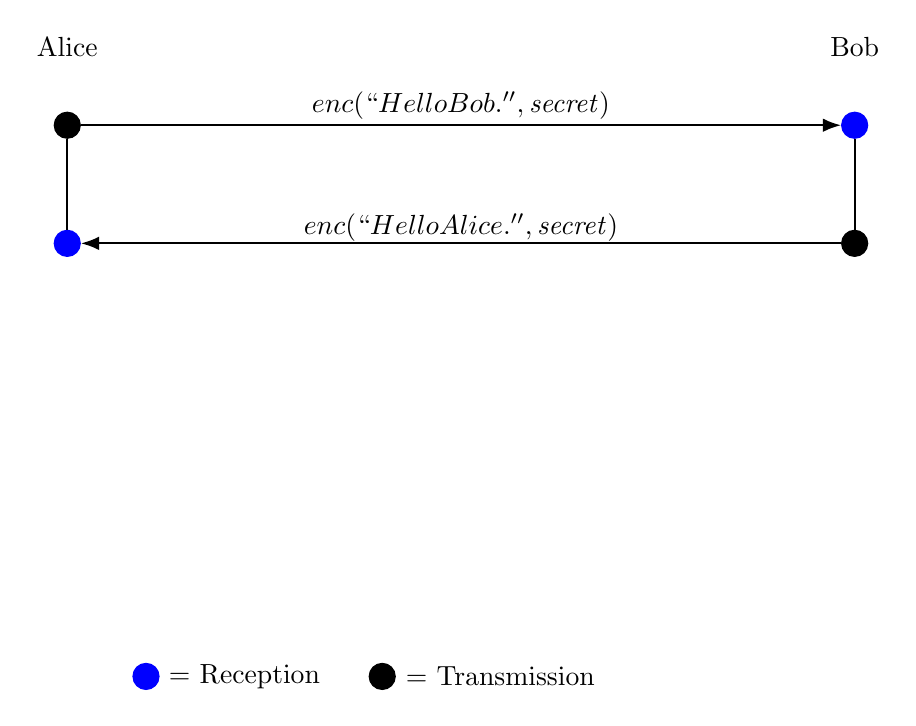
\begin{tikzpicture}
    \node at (0,8) {Alice};
    \node at (10,8) {Bob};
    \node[shape=circle,draw=blue, fill=blue] at (1,0) {};
    \node at (2.25,0) {= Reception};
    \node[shape=circle,draw=black, fill=black] at (4,0) {};
    \node at (5.5,0) {= Transmission};


    \node[shape=circle,draw=black, fill=black] (1) at (0,7) {};
    \node[shape=circle,draw=blue, fill=blue] (2) at (10,7) {};
    \path [saiarrow](1) edge (2);
    
    \node at (5,7.25) {\(enc(\text{``Hello Bob.''}, \mathit{secret})\)};
    
    \node[shape=circle,draw=black, fill=black] (3) at (10,5.5) {};
    \node[shape=circle,draw=blue, fill=blue] (4) at (0,5.5) {};
    
    \path [-,thick](3) edge (2);
    \path [saiarrow](3) edge (4);
    \path [-,thick](1) edge (4);
    
    \node at (5,5.7) {\(enc(\text{``Hello Alice.''},\mathit{secret})\)};
\end{tikzpicture}
\end{frame}

\begin{frame}\frametitle{Asymmetric encryption}
\pause
Let \(m\) be a message, \(pub_k,priv_k\) be a public-private key pair, and \(c\) be ciphertext.
\pause
\begin{definition}[Encryption]
A function \(f\) is \emph{encrypting} if:
\[
f(m,pub_k) = c
\]
\end{definition}
\pause
\begin{definition}[Decryption]
A function \(f\) is \emph{decrypting} if:
\[
f(c,priv_k) = m
\]
\end{definition}
\pause
Common asymmetric key algorithms include RSA, ElGamal, and Elliptic Curve.
\end{frame}

\begin{frame}\frametitle{Asymmetric Encryption Diagram}
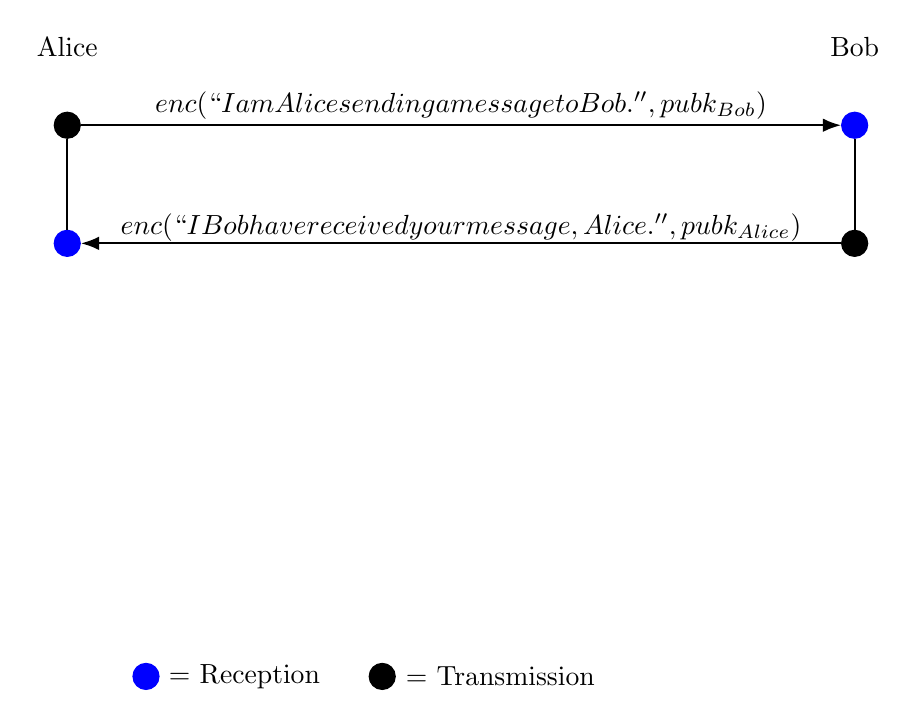
\begin{tikzpicture}
    \node at (0,8) {Alice};
    \node at (10,8) {Bob};
    \node[shape=circle,draw=blue, fill=blue] at (1,0) {};
    \node at (2.25,0) {= Reception};
    \node[shape=circle,draw=black, fill=black] at (4,0) {};
    \node at (5.5,0) {= Transmission};


    \node[shape=circle,draw=black, fill=black] (1) at (0,7) {};
    \node[shape=circle,draw=blue, fill=blue] (2) at (10,7) {};
    \path [saiarrow](1) edge (2);
    
    \node at (5,7.25) {\(enc(\text{``I am Alice sending a message to Bob.''}, pubk_{Bob})\)};
    
    \node[shape=circle,draw=black, fill=black] (3) at (10,5.5) {};
    \node[shape=circle,draw=blue, fill=blue] (4) at (0,5.5) {};
    
    \path [-,thick](3) edge (2);
    \path [saiarrow](3) edge (4);
    \path [-,thick](1) edge (4);
    
    \node at (5,5.7) {\(enc(\text{``I Bob have received your message, Alice.''},pubk_{Alice})\)};
\end{tikzpicture}
\end{frame}

\begin{frame}\frametitle{Signing}
\pause
Let \(m\) be a message, \(pub_k,priv_k\) be a public-private key pair, and \(c\) be ciphertext.
\pause
\begin{definition}[Signing]
A function \(f\) produces a \emph{signature} if:
\[
f(m,priv_k) = c
\]
\end{definition}
\pause
\begin{definition}[Verifying]
A function \(f\) can be used to \emph{verify} if:
\[
f(c,pub_k) = m
\]
\end{definition}
\pause
More or less the same as the asymmetric algorithms.
\end{frame}

\begin{frame}\frametitle{Signing Diagram}
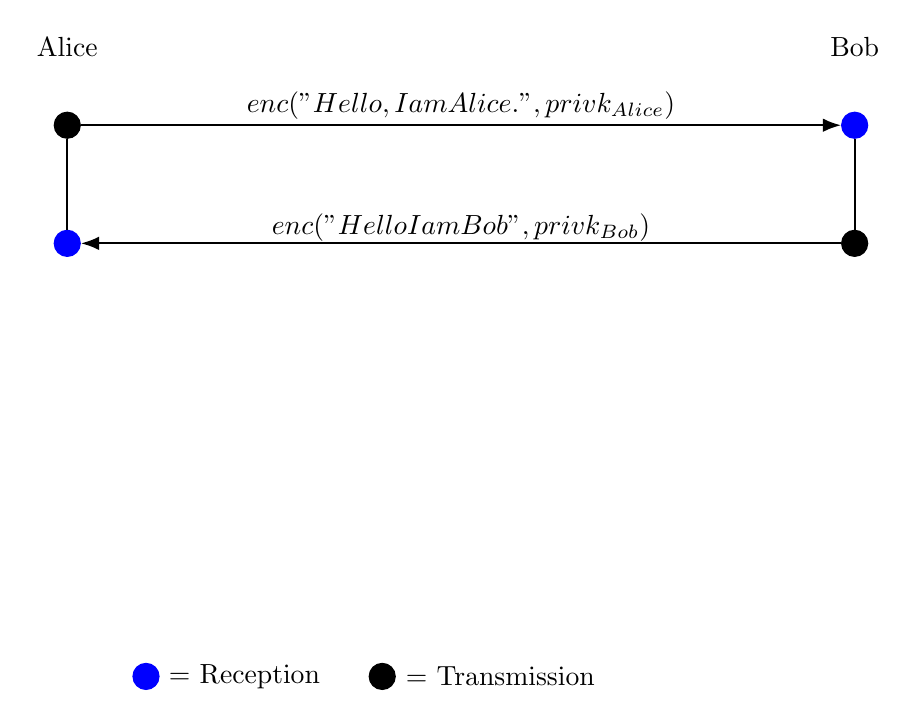
\begin{tikzpicture}
    \node at (0,8) {Alice};
    \node at (10,8) {Bob};
    \node[shape=circle,draw=blue, fill=blue] at (1,0) {};
    \node at (2.25,0) {= Reception};
    \node[shape=circle,draw=black, fill=black] at (4,0) {};
    \node at (5.5,0) {= Transmission};


    \node[shape=circle,draw=black, fill=black] (1) at (0,7) {};
    \node[shape=circle,draw=blue, fill=blue] (2) at (10,7) {};
    \path [saiarrow](1) edge (2);
    
    \node at (5,7.25) {\(enc(\text{"Hello, I am Alice."}, privk_{Alice})\)};
    
    \node[shape=circle,draw=black, fill=black] (3) at (10,5.5) {};
    \node[shape=circle,draw=blue, fill=blue] (4) at (0,5.5) {};
    
    \path [-,thick](3) edge (2);
    \path [saiarrow](3) edge (4);
    \path [-,thick](1) edge (4);
    
    \node at (5,5.7) {\(enc(\text{"Hello I am Bob"},privk_{Bob})\)};
\end{tikzpicture}
\end{frame}

\begin{frame}\frametitle{Hashing}
\pause
Let \(m\) be a message, \(md\) be a message digest.
\pause
\begin{definition}[Hashing]
A function \(h\) is called an \emph{hash function} if:
\begin{enumerate}
\item \(h(m) = md\)
\item It is impractical to determine \(m\) given \(md\).
\item Collision Resistance: It is infeasible to find \(m_1,m_2\) such that \(h(m_1) = h(m_2)\).
\end{enumerate}
\end{definition}
\pause
Common hash functions include the MD family, SHA family, and Skein.
\end{frame}

\begin{frame}\frametitle{Hashing Diagram}
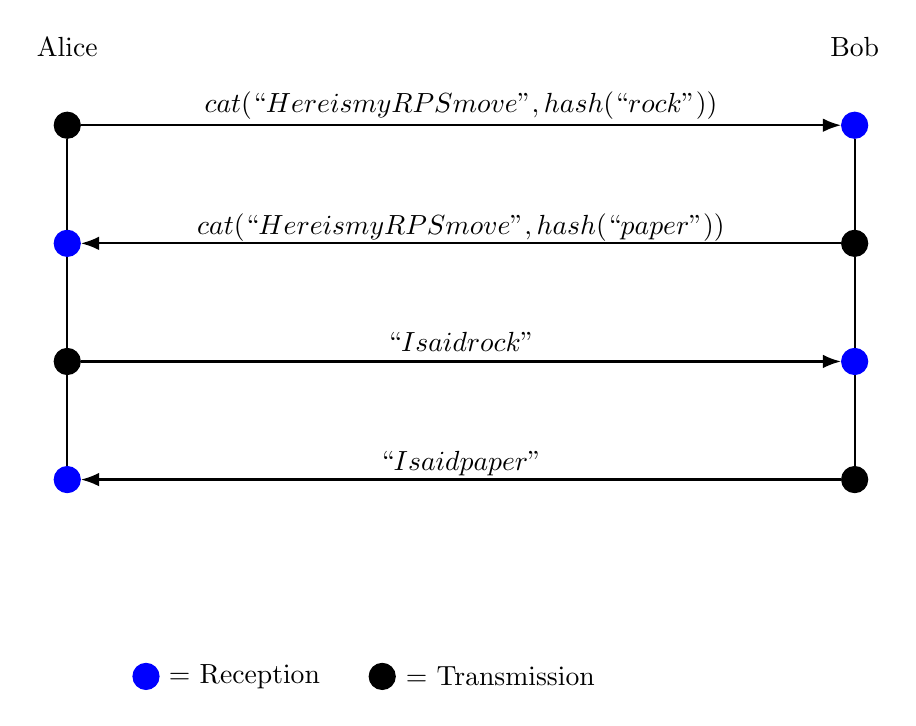
\begin{tikzpicture}
    \node at (0,8) {Alice};
    \node at (10,8) {Bob};
    \node[shape=circle,draw=blue, fill=blue] at (1,0) {};
    \node at (2.25,0) {= Reception};
    \node[shape=circle,draw=black, fill=black] at (4,0) {};
    \node at (5.5,0) {= Transmission};


    \node[shape=circle,draw=black, fill=black] (1) at (0,7) {};
    \node[shape=circle,draw=blue, fill=blue] (2) at (10,7) {};
    \path [saiarrow](1) edge (2);
    
    \node at (5,7.25) {\(cat(\text{``Here is my RPS move"}, hash(\text{``rock"}))\)};
    
    \node[shape=circle,draw=black, fill=black] (3) at (10,5.5) {};
    \node[shape=circle,draw=blue, fill=blue] (4) at (0,5.5) {};
    
    \path [-,thick](3) edge (2);
    \path [saiarrow](3) edge (4);
    \path [-,thick](1) edge (4);
    
    \node at (5,5.7) {\(cat(\text{``Here is my RPS move"}, hash(\text{``paper"}))\)};

    \node[shape=circle,draw=black, fill=black] (5) at (0,4) {};
    \node[shape=circle,draw=blue, fill=blue] (6) at (10,4) {};
    \path [saiarrow](5) edge (6);

    \path [-,thick](3) edge (6);
    \path [-,thick](4) edge (5);
    
    \node at (5,4.25) {\(\text{``I said rock"}\)};
    
    \node[shape=circle,draw=black, fill=black] (7) at (10,2.5) {};
    \node[shape=circle,draw=blue, fill=blue] (8) at (0,2.5) {};
    
    \path [-,thick](7) edge (6);
    \path [saiarrow](7) edge (8);
    \path [-,thick](5) edge (8);
    
    \node at (5,2.7) {\(\text{``I said paper"}\)};
\end{tikzpicture}
\end{frame}

\begin{frame}\frametitle{Nonces}
\begin{definition}[Nonce]
A nonce is a \emph{fresh, random} number that is generated by a principal.
Nonces are used to make sure that communication is happening with the right person at the right time.
\pause

We can also use them to make sure that the hash property of invertibility is not easily compromisable.
\end{definition}

\end{frame}

\begin{frame}\frametitle{Hashing Diagram (fixed)}
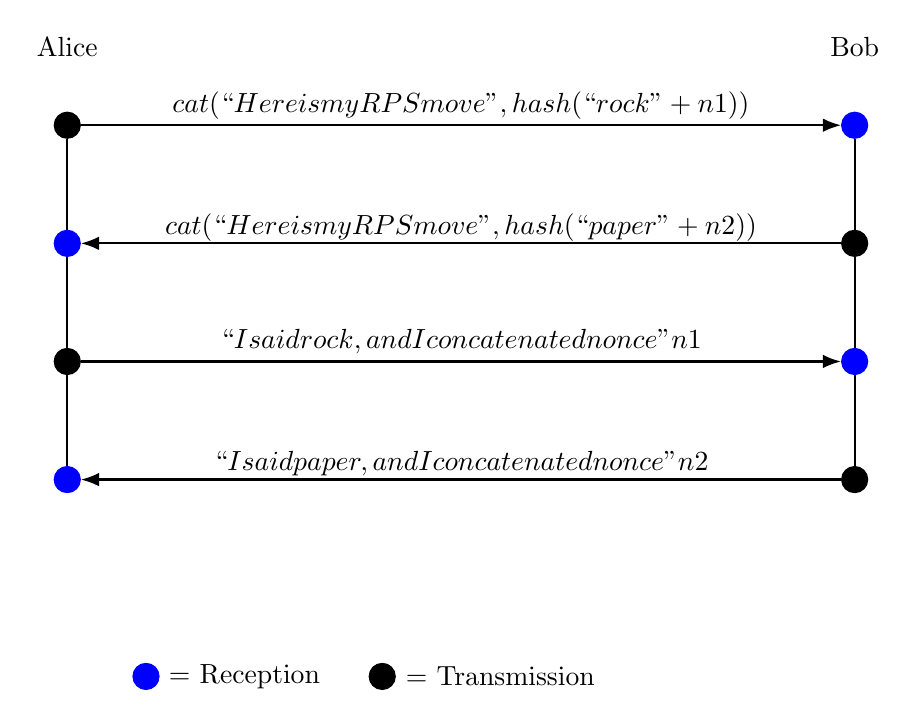
\begin{tikzpicture}
    \node at (0,8) {Alice};
    \node at (10,8) {Bob};
    \node[shape=circle,draw=blue, fill=blue] at (1,0) {};
    \node at (2.25,0) {= Reception};
    \node[shape=circle,draw=black, fill=black] at (4,0) {};
    \node at (5.5,0) {= Transmission};


    \node[shape=circle,draw=black, fill=black] (1) at (0,7) {};
    \node[shape=circle,draw=blue, fill=blue] (2) at (10,7) {};
    \path [saiarrow](1) edge (2);
    
    \node at (5,7.25) {\(cat(\text{``Here is my RPS move"}, hash(\text{``rock"} + n1))\)};
    
    \node[shape=circle,draw=black, fill=black] (3) at (10,5.5) {};
    \node[shape=circle,draw=blue, fill=blue] (4) at (0,5.5) {};
    
    \path [-,thick](3) edge (2);
    \path [saiarrow](3) edge (4);
    \path [-,thick](1) edge (4);
    
    \node at (5,5.7) {\(cat(\text{``Here is my RPS move"}, hash(\text{``paper"} + n2))\)};

    \node[shape=circle,draw=black, fill=black] (5) at (0,4) {};
    \node[shape=circle,draw=blue, fill=blue] (6) at (10,4) {};
    \path [saiarrow](5) edge (6);

    \path [-,thick](3) edge (6);
    \path [-,thick](4) edge (5);
    
    \node at (5,4.25) {\(\text{``I said rock, and I concatenated nonce" } n1\)};
    
    \node[shape=circle,draw=black, fill=black] (7) at (10,2.5) {};
    \node[shape=circle,draw=blue, fill=blue] (8) at (0,2.5) {};
    
    \path [-,thick](7) edge (6);
    \path [saiarrow](7) edge (8);
    \path [-,thick](5) edge (8);
    
    \node at (5,2.7) {\(\text{``I said paper, and I concatenated nonce" } n2\)};
\end{tikzpicture}
\end{frame}

\begin{frame}\frametitle{Cryptographic Primitives Summary}
\begin{itemize}
\item Asymmetric keys: Used for exchanging information where both parties do not have a shared secret. Also used for signatures. Can be time consuming to compute.
\item Symmetric keys: Used for exchanging information where both parties can preshare a shared secret. Easier to compute.
\item Hashing: Creates a fixed-length deterministic fingerprint of some information.
\end{itemize}
\end{frame}

\begin{frame}\frametitle{CPSA Term Algebra}
\begin{itemize}
\item A term algebra consists of: 
\begin{itemize}
    \item  A set of elements called terms, built recursively from a base set of variables and constants by applying functions. % SM: can we talk about what these are in CPSA? (like say "the base set being an arbitrary message").  also is recursively correct? isnt it just a subtype relation? Maybe polymorphically
    \item The application functions themselves, which are what make it an algebra rather than just a set.
\end{itemize}
\item The variables and constants within our term algebra fall into "sorts," similar to data types in programming languages.
\item The actions we talked about (hashing, encryption, public keys) are functions in this term algebra.
\end{itemize}
\end{frame}

\begin{frame}\frametitle{Homework}
\pause
\begin{center}
{\Huge Design a protocol}
\end{center}
\pause
\begin{enumerate}
\item Two parties: Alice and Bob
\item Agree to meet at a specific time and place
\item Mitigate the Dolev-Yao adversary.
\end{enumerate}
\end{frame}

\begin{frame}\frametitle{Survey}
\begin{itemize}
\item A survey will be administered after each of these lectures.
\item These surveys include objective questions about the lecture, as long as feedback about how us lecturers delivered it. 
\item  Surveys are due by the start of the next session (in this case Thursday at 6:00pm). We encourage you to complete them as soon as possible while the information is fresh.
\end{itemize}

\begin{figure}
    \centering
    \includegraphics[width=0.5\linewidth]{qr-codes/surveyQuiz1.png}
    \caption{Enter Caption}
    \label{fig:placeholder}
\end{figure}

\end{frame}
\end{document}